\newpage
\section{Super Kaleidoscopes}

In this activity, we're going to investigate a different way to draw
stars.

\begin{prob}
Apply every element of
$\{\mat{R}_{0},\mat{R}_{90},\mat{R}_{180},\mat{R}_{270}\}$ to the
picture below. What picture do you get?
\[
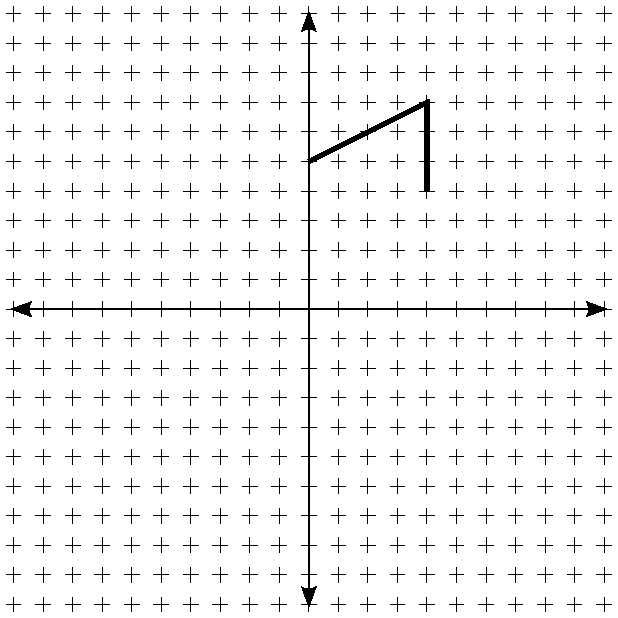
\includegraphics{../graphics/PlaneOrbit1.pdf}
\]
This is called the \textbf{orbit}\index{orbit} of
$\{\mat{R}_{0},\mat{R}_{90},\mat{R}_{180},\mat{R}_{270}\}$ on the
figure above.
\end{prob}

\vfill

\break

\begin{prob}
Apply every element of $\{\mat{F}_{x=0}, \mat{F}_{y=0}, \mat{F}_{x=y},\mat{F}_{x=-y}\}$ to the picture below. What picture do
you get?
\[
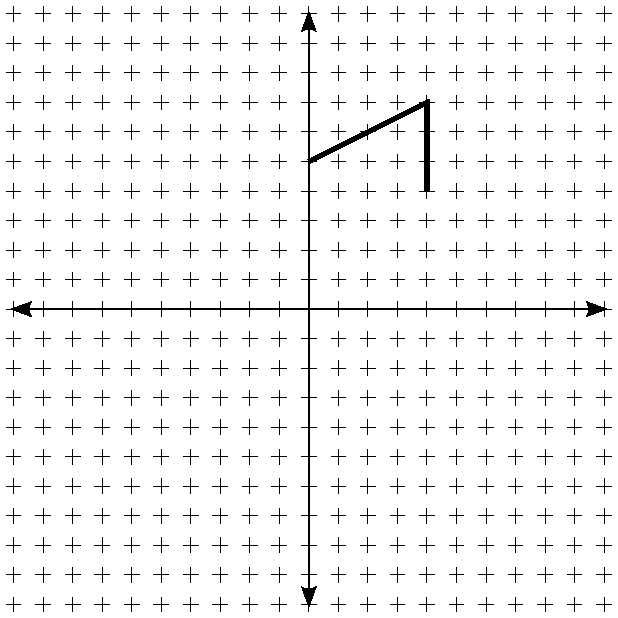
\includegraphics{../graphics/PlaneOrbit1.pdf}
\]
\end{prob}

\vfill

\break

\begin{prob}
Apply every element of $\{\mat{R}_{0},\mat{R}_{90},\mat{R}_{180},\mat{R}_{270}\}$ to the picture below. What picture do
you get?
\[
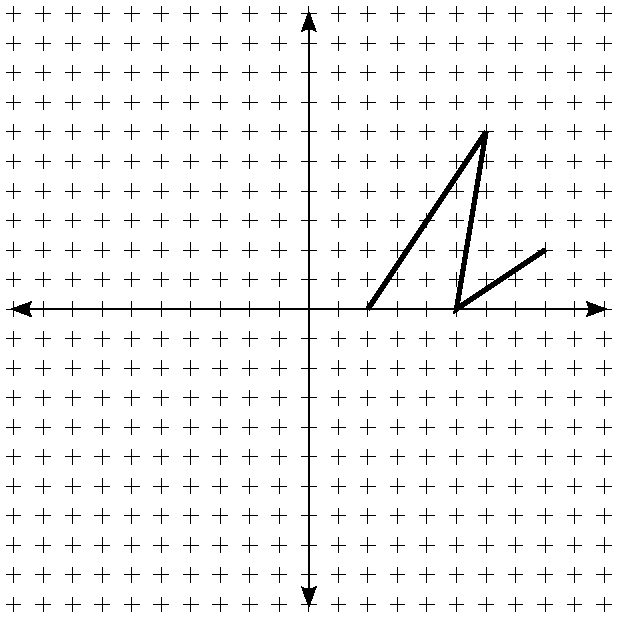
\includegraphics{../graphics/PlaneOrbit2.pdf}
\]
\end{prob}

\vfill

\break

\begin{prob}
Apply every element of
$\{\mat{F}_{x=0}, \mat{F}_{y=0}, \mat{F}_{x=y},\mat{F}_{x=-y}\}$ to
the picture below. What picture do you get?
\[
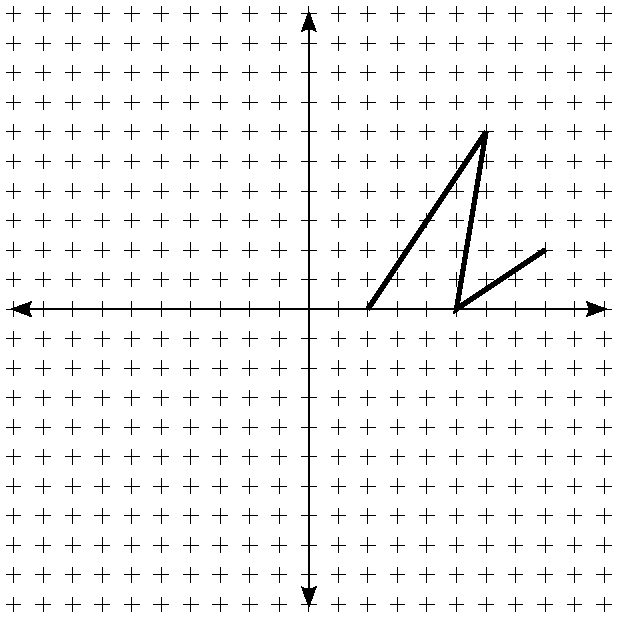
\includegraphics{../graphics/PlaneOrbit2.pdf}
\]
\end{prob}

\vfill


